\documentclass{standalone}
\usepackage{tikz}
\usetikzlibrary{calc, shapes, patterns}

\begin{document}
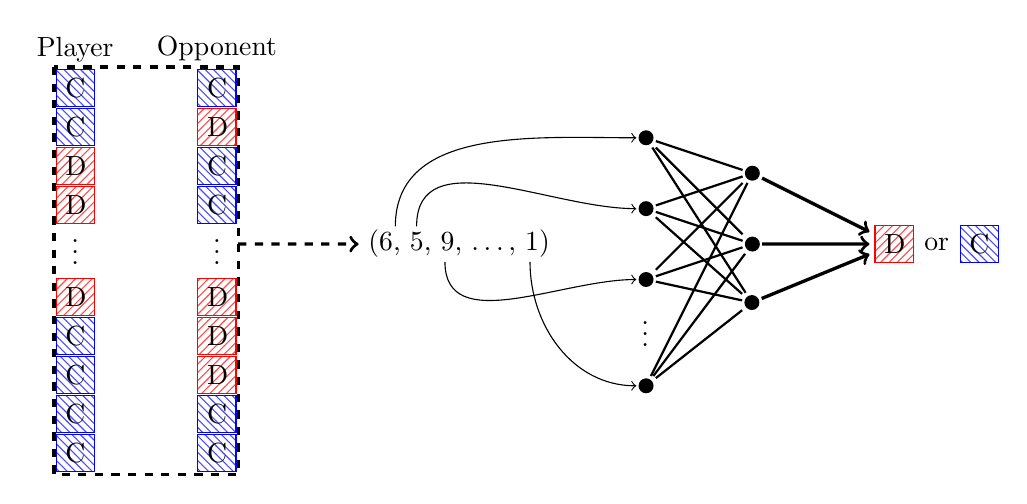
\begin{tikzpicture}[scale=.9]
    \tikzstyle{cooperator} = [rectangle, pattern=north west lines, pattern
        color=blue!70, draw=blue, text width=.25cm, outer sep = 2pt]
    \tikzstyle{defector} = [rectangle, pattern=north east lines, pattern
        color=red!70, draw=red, text width=.25cm, outer sep = 2pt]


    % Histories ----------------------------------------
    \node (A) at (-.5, 0) {Player};
    \node (A1) at ($(A) + (0, -.55)$) [cooperator] {C};
    \node (A2) at ($(A1) + (0, -.55)$) [cooperator] {C};
    \node (A3) at ($(A2) + (0, -.55)$) [defector] {D};
    \node (A4) at ($(A3) + (0, -.55)$) [defector] {D};
    \node (A5) at ($(A4) + (0, -.55)$) {$\vdots$};
    \node (A6) at ($(A5) + (0, -.75)$) [defector] {D};
    \node (A7) at ($(A6) + (0, -.55)$) [cooperator] {C};
    \node (A8) at ($(A7) + (0, -.55)$) [cooperator] {C};
    \node (A9) at ($(A8) + (0, -.55)$) [cooperator] {C};
    \node (A10) at ($(A9) + (0, -.55)$) [cooperator] {C};


    \node (B) at ($(A) + (2, 0)$) {Opponent};
    \node (B1) at ($(B) + (0, -.55)$) [cooperator] {C};
    \node (B2) at ($(B1) + (0, -.55)$) [defector] {D};
    \node (B3) at ($(B2) + (0, -.55)$) [cooperator] {C};
    \node (B4) at ($(B3) + (0, -.55)$) [cooperator] {C};
    \node (B5) at ($(B4) + (0, -.55)$) {$\vdots$};
    \node (B6) at ($(B5) + (0, -.75)$) [defector] {D};
    \node (B7) at ($(B6) + (0, -.55)$) [defector] {D};
    \node (B8) at ($(B7) + (0, -.55)$) [defector] {D};
    \node (B9) at ($(B8) + (0, -.55)$) [cooperator] {C};
    \node (B10) at ($(B9) + (0, -.55)$) [cooperator] {C};
    % ---------------------------------------------------

    % Identifying inputs --------------------------------
    \draw[very thick, black, dashed] ($(A1) + (-.3, .3)$)  rectangle ($(B10) + (.3, -.3)$);

    % Strategy inputs
    \node (input_vector) at ($(B5) + (2, 0)$) [right] {(6, 5, 9, \dots, 1)};

    \draw [very thick, black, dashed, ->] ($(B5) + (.3, 0)$) -- (input_vector);


    % Neural network

    \node (in1) at ($(input_vector) + (2.5, 1.5)$) [right] {};
    \fill (in1) circle[radius=3pt];
    \node (in2) at ($(input_vector) + (2.5, .5)$) [right] {};
    \fill (in2) circle[radius=3pt];
    \node (in3) at ($(input_vector) + (2.5, -.5)$) [right] {};
    \fill (in3) circle[radius=3pt];

    \node (in4) at ($(input_vector) + (2.625, -1.15)$) {$\vdots$};

    \node (in5) at ($(input_vector) + (2.5, -2)$) [right] {};
    \fill (in5) circle[radius=3pt];

    % Inputs

    \draw [->] ($(input_vector) + (-.9, .25)$) to [in=180, out=90] (in1);
    \draw [->] ($(input_vector) + (-.6, .25)$) to [in=180, out=90] (in2);
    \draw [->] ($(input_vector) + (-.2, -.25)$) to [in=180, out=-90] (in3);
    \draw [->] ($(input_vector) + (1, -.25)$) to [in=180, out=-90] (in5);

    \node (mid1) at ($(in1)!0.5!(in2) + (1.5, 0)$) {};
    \fill (mid1) circle[radius=3pt];
    \node (mid2) at ($(in2)!0.5!(in3) + (1.5, 0)$) {};
    \fill (mid2) circle[radius=3pt];
    \node (mid3) at ($(in3)!0.5!(in4) + (1.5, 0)$) {};
    \fill (mid3) circle[radius=3pt];

    \draw [thick] (in1) -- (mid1);
    \draw [thick] (in1) -- (mid2);
    \draw [thick] (in1) -- (mid3);

    \draw [thick] (in2) -- (mid1);
    \draw [thick] (in2) -- (mid2);
    \draw [thick] (in2) -- (mid3);

    \draw [thick] (in3) -- (mid1);
    \draw [thick] (in3) -- (mid2);
    \draw [thick] (in3) -- (mid3);

    \draw [thick] (in5) -- (mid1);
    \draw [thick] (in5) -- (mid2);
    \draw [thick] (in5) -- (mid3);

    % output
    \node (output) at ($(mid2) + (2, 0)$) [defector] {D};
    \node (or) at ($(output) + (.6, 0)$) {or};
    \node at ($(or) + (.6, 0)$) [cooperator] {C};

    \draw [->, very thick] (mid1) -- (output);
    \draw [->, very thick] (mid2) -- (output);
    \draw [->, very thick] (mid3) -- (output);
\end{tikzpicture}
\end{document}
